%---------- Quinto Capítulo: Resultados ----------

\chapter{Resultados} %5 --- 10 pags

Com o conjunto de ferramentas desenvolvidos neste projeto aliado a uma base de vídeos originais é possível produzir e avaliar uma nova e diversificada base com vídeos degradados em qualidade e quantitade variável.
Neste Capítulo serão verificados os resultados obtidos a partir do processamento de vídeos efuados por estas ferramentas. Primeiramente uma avaliação subjetiva das ferramentas de degradação utilizando diversas amostras retiradas de um vídeo da base. A seguir é feita a validação dos resultados obtidos pela ferramenta de métricas objetivas, tomando como base (base do wyllian!!).
Por fim é feita uma análise das notas de avaliação objetivas buscando mensurar o impacto que determinadas degradações podem ter sobre um conjunto de vídeos com características diferentes.

\section{Validação das Ferramentas de Artefatos}

Foram efetuados diversos processos de degradação sobre o vídeo bus, obtido em \cite{tracevideoseq},  empregando diferentes paramêtros a cada processamento e para cada ferramenta, buscando identificar visualmente e os artefatos produzidos e determinar sua semelhanca com os vistos em situações reais.

A primeira ferramenta a ser avaliada é a \emph{block}.
Para a avaliação foram gerados 14 vídeos onde é efetuado o processo de blocagem, com blocos 8x8, de forma integral --- para todos os blocos em todos os quadros. A cada novo vídeo gerado foram eliminadas de forma cumulativa diagonais na matriz resultante da transformação DCT, partindo da diagonal mais inferior, até que no último vídeo restasse somente a componente DC da transformada. 
Na Figura \ref{fig:blockbus} são apresentados recortes de 160 por 160 \emph{pixels} a partir da posição 64x160 retirados do frame de número 60 de cada um dos 14 vídeos obtidos, sendo que o primeiro recorte foi obtido do vídeo original.

Observando os recortes com cautela é possível notar degradações extremamente sutis a partir do recorte \emph{07}, verificadas com mais facilidade nos arredores da publicidade na lateral do ônibus.No recorte de número \emph{10} as regiões de alta frequência da imagem denunciam degradações mais acentuadas, e no \emph{11} já não é mais possível identificar o que está escrito na placa de publicidade, embora ainda seja razoavél identificar a cena da imagem.
Nos três recortes seguintes o efeito de blocagem passa a tomar conta da imagem e apenas objetos de grande escala passam a ser identificávies, sendo que no recorte de número \emph{14} até mesmo a identificação da cena fica prejudicada.

\begin{figure}[!htb]
	\centering
	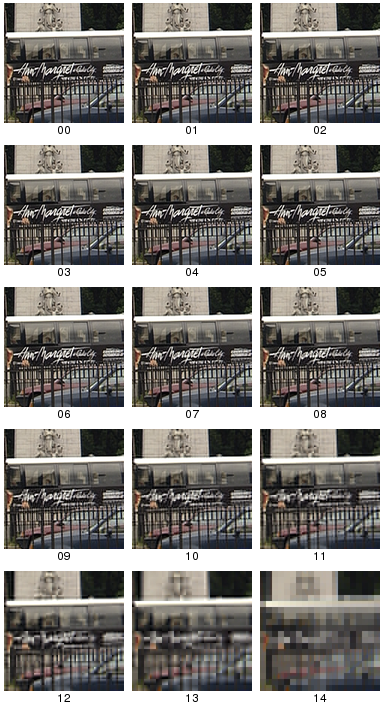
\includegraphics[width=0.8\textwidth]{./imgs/blockbus.png}
	\caption{Sequência de degradações eliminando gradativamente diagonais da DCT.}
	\label{fig:blockbus}
	\fonte{Autoria Própria.}
\end{figure}

Para a avaliação da ferramenta \emph{blur} foram feitas duas sequências de testes, a primeira delas utilizando o filtro de médias e a segunda utilizando o filtro da mediana.
Em cada um dos testes foram utilizadas máscaras matriciais de tamanhos 3x3, 5x5 e 7x7. Nas Figuras \ref{fig:bluraverage} e \ref{fig:blurmedian} são apresentados recortes de 160 por 160 \emph{pixels} a partir da posição 64x160 retirados do frame número 60 de cada vídeo.

\begin{figure}[!htb]
	\centering
	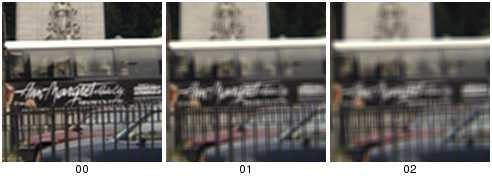
\includegraphics[width=0.9\textwidth]{./imgs/bluraverage.png}
	\caption{Sequência de borramentos aplicando filtro da média com matrizes (00) 3x3, (01) 5x5, (02) 7x7.}
	\label{fig:bluraverage}
	\fonte{Autoria Própria.}
\end{figure}

\begin{figure}[!htb]
	\centering
	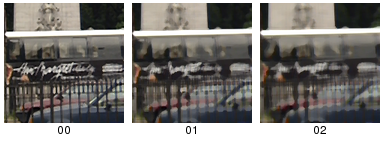
\includegraphics[width=0.9\textwidth]{./imgs/blurmedian.png}
	\caption{Sequência de borramentos aplicando filtro da mediana com matrizes (00) 3x3, (01) 5x5, (02) 7x7.}
	\label{fig:blurmedian}
	\fonte{Autoria Própria.}
\end{figure}

Na validação visual da ferramenta \emph{raffle} foi gerado um arquivo de sorteio contendo 5 mil elementos.
A distribuição no tempo foi configurada como triangular no intervalo de 0 a 10 com pico no frame 5, sendo que a duração de cada artefato foi distribuída uniformemente no intervalo de 1 a 3 frames.
Já a distribuição no espaço foi uniforme em toda a largura e altura do frame. 
A figura \ref{fig:busraffle} mostra a sequencia de recortes retirados dos 11 frames contendo blocos gerados a partir do arquivo raffle obtido com a configuração acima, onde para facilitar a visualização foi elimanada a componente DC da DCT para cada bloco sorteado.

\begin{figure}[!htb]
	\centering
	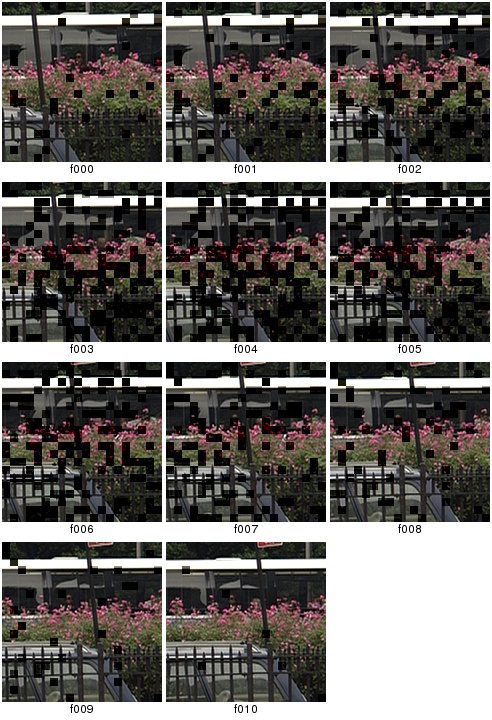
\includegraphics[width=0.8\textwidth]{./imgs/busraffle.png}
	\caption{Sequência de frames degradados a partir de um arquivo gerado pela ferramenta \emph{raffle}.}
	\label{fig:busraffle}
	\fonte{Autoria Própria.}
\end{figure}

Para o processo de validação da ferramenta \emph{netsim} foi necessário obter um vídeo encapsulado em um TS, para isso foi utilizada a ferramenta ffmpeg para converter o vídeo bus para a codificação MPEG-2 encapsulado em um TS com o seguinte comando:

{
	\centering
	\texttt{ffmpeg -i \emph{arquivo\_de\_entrada} -s cif -sameq -f mpegts -vcodec mpeg2video \emph{arquivo\_de\_saída}}
}

O TS resultante foi então processado pela ferramenta, configurada para fazer os seguintes descartes:

\begin{center}
	\texttt{10 100
	1000 10
	100 10
	1 10
	100 50}
\end{center}

A figura \ref{fig:netsim} contém amostras retiradas dos frames 1, 9 e 40, onde podem ser verificados artefatos como \emph{jerkiness}, \emph{blocking} e \emph{bleeding}.

\begin{figure}[!htb]
	\centering
	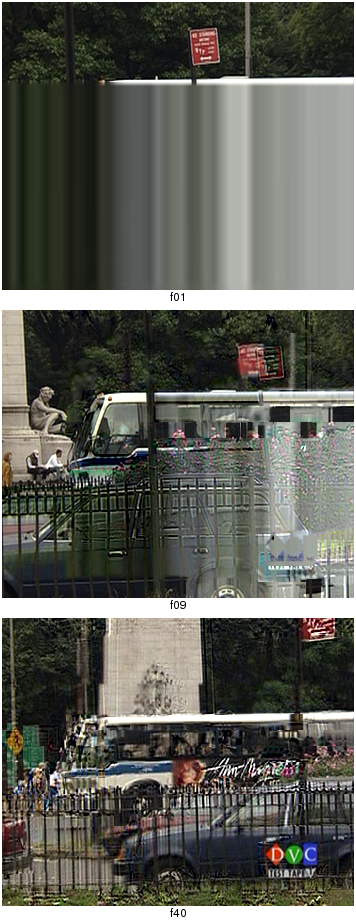
\includegraphics[height=0.9\textheight]{./imgs/netsimresult.png}
	\caption{Amostra de artefados obtidos com a ferramenta \emph{netsim}}
	\label{fig:netsim}
	\fonte{Autoria Própria.}
\end{figure}

\section{Validação da Ferramenta de Métricas}

Para validação dos valores de MSE, PSNR e MSSIM calculados pela ferramenta \emph{metric} foi feita a comparação destes com os obtidos pela ferramenta MSU \emph{Video Quality Measurement Tool}.
Esta última foi desenvolvida pelo grupo do laboratório \emph{Graphics and Media Lab} da \emph(Moscow State University) (MSU) e possui a implementação de diversas métricas objetivas \cite{moscowuniversity}.
%TODO base de videos das metricas
Foram utilizados 5 vídeos diferentes, e os respoectivos vídeos degradados,  obtidos em \cite{}. Os resultados das comparações se encontram nas tabelas \ref{res:mse}, \ref{res:psnr} e \ref{res:mssim}.

\begin{table}[!htb]
	\centering
	\caption{Comparação dos resultados de PSNR.}
	\label{res:psnr}
	\begin{tabular}{lccc}
		\hline
		Video	 & MSU	 & SASQV2	 & Erro (\%) \\ \hline
		aircraft	 & 23.49501 & 23.49501 & 0.00000	 \\ 
		liberty	 & 29.21472 & 29.21472 & 0.00000	 \\ 
		ship	 & 25.56667 & 25.56667 & 0.00000	 \\ 
		stockholm & 18.90942 & 18.90942 & 0.00000	 \\ 
		whale	 & 20.59830 & 20.59830 & 0.00000	 \\
	\hline
	\end{tabular}
	\fonte{Autoria pŕopria}
\end{table}

\begin{table}[!htb]
	\centering
	\caption{Comparação dos resultados de MSE.}
	\label{res:mse}
	\begin{tabular}{lccc}
	\hline
	Video	 & MSU	 & SASQV2	 & Erro (\%) \\ \hline
	aircraft	 & 290.78970 & 290.78970 & 0.00000	 \\ 
	liberty	 & 77.91273	 & 77.91273	 & 0.00000	 \\ 
	ship	 & 180.47363 & 180.47362 & -0.00001 \\ 
	stockholm & 835.86987 & 835.86987 & 0.00000	 \\ 
	whale	 & 566.53094 & 566.56611 & 0.00621	 \\
	\hline
	\end{tabular}
	\fonte{Autoria própria}
\end{table}

\begin{table}[!htb]
	\centering
	\caption{Comparação dos resultados de MSSIM.}
	\label{res:mssim}
	\begin{tabular}{lccc}
	\hline
	Video	 & MSU	 & SASQV2	 & Erro (\%) \\ \hline
	aircraft	 & 0.79457 & 0.80723 & 1.59306	 \\
	liberty	 & 0.85415 & 0.85627 & 0.24843	 \\
	ship	 & 0.70462 & 0.70628 & 0.23530	 \\ 
	stockholm & 0.42486 & 0.43327 & 1.97948	 \\ 
	whale	 & 0.81918 & 0.82240 & 0.39320	 \\
	\hline
	\end{tabular}
	\fonte{Autoria própria.}
\end{table}

Observando os resultados para MSE e PSNR pode-se dizer que os resultados são fiéis e que a ferramenta se comporta como o esperado.

\section{Análise de Impacto Sobre Métricas Objetivas}

\section{Resumo e Conclusão do Capítulo}
